\section{Domain Analysis}

\subsection{User Interfaces and Input Devices}

% Before diving in the deeps of real-time communication over the Web, it is necessary to review the path that people took in order to interact with computers in the first place.

At the very beginning of the computer era, the devices that we now know as
PCs, laptops and tablets were immense pieces of machinery that occupied entire
laboratories and only highly qualified individuals had access to them. These
machines where developed in order to perform various numerical problems by
executing digital computations. As the saying goes, a machine can only do what
a man tells it to do, so engineers had to come up with different means to set
tasks for these electronic beasts, that is, a need for \emph{user interfaces}
arouse. Operators used large stacks of punched cards to feed instructions and
data sets to computers. These punched cards in turn where created using
specialized devices that also required some knowledge in the field. Over all
it was a complex process that couldn't be easily grasped by an ordinary
persons. At that time, however, the majority of computer user had PhDs and
were trained to perform these very tasks so the difficulty of communicating
with machines wasn't really a great problem.

% picture of ENIAC maybe

In time, the interest towards computers grew bigger among enthusiasts while
the devices themselves where becoming smaller and smaller, eventually giving
birth to the term of 'microcomputer'. Among the first microcomputers to get
widespread popularity was the critically acclaimed Altair 8080 which
represented a box with lights and switches on the front panel that where used
to feed data and instructions into the computer and read the results back from
it.

% picture of Altair 8080 front panel

As more hobbyists took a hold of such devices people discovered many uses for
them beyond that of performing various mathematical operations. They learned
how to connect teletypes to computers and this way the later got an interface
that is familiar to all of us today, a keyboard. For some time people
interacted with computers using command lines, but with the development of
computer graphics and the creation of graphical user interfaces, a need for a
new kind of controller appeared, specifically the need for a pointing device.
Since then, a standard personal computer included a mouse and a keyboard among
it's peripheral devices.

\subsubsection{Input Devices for Gaming}

On the other hand, the development of input devices never stopped with the
creation of the mouse and keyboard. A wealth of specialized devices was
created to perform tasks that were specific to a particular use of the
computer. One of the most notable fields that was moving the development of
specialized peripherals was and still is the \emph{game development industry}.
During the years, various types of controllers were developed, some of them
are listed below:

\begin{description}

    \item [Gamepad] is a general-purpose gaming device that is used as a
        controller for a wide range of game genres, from arcades and fighting
        games to role-playing titles and action third-person shooters.

    \item [Joystick] is a specialized controller that is often used in flight
        simulation games, although its use can be extended far beyond gaming, for such
        purposes as remote control of a robot arm in a warehouse.

    \item [Steering Wheel] is used to provide almost authentic driving
        experience in racing video games.

\end{description}


\begin{figure}[!ht]
    \centering
    \subfloat[Gamepad\label{fig:gamepad}]{
      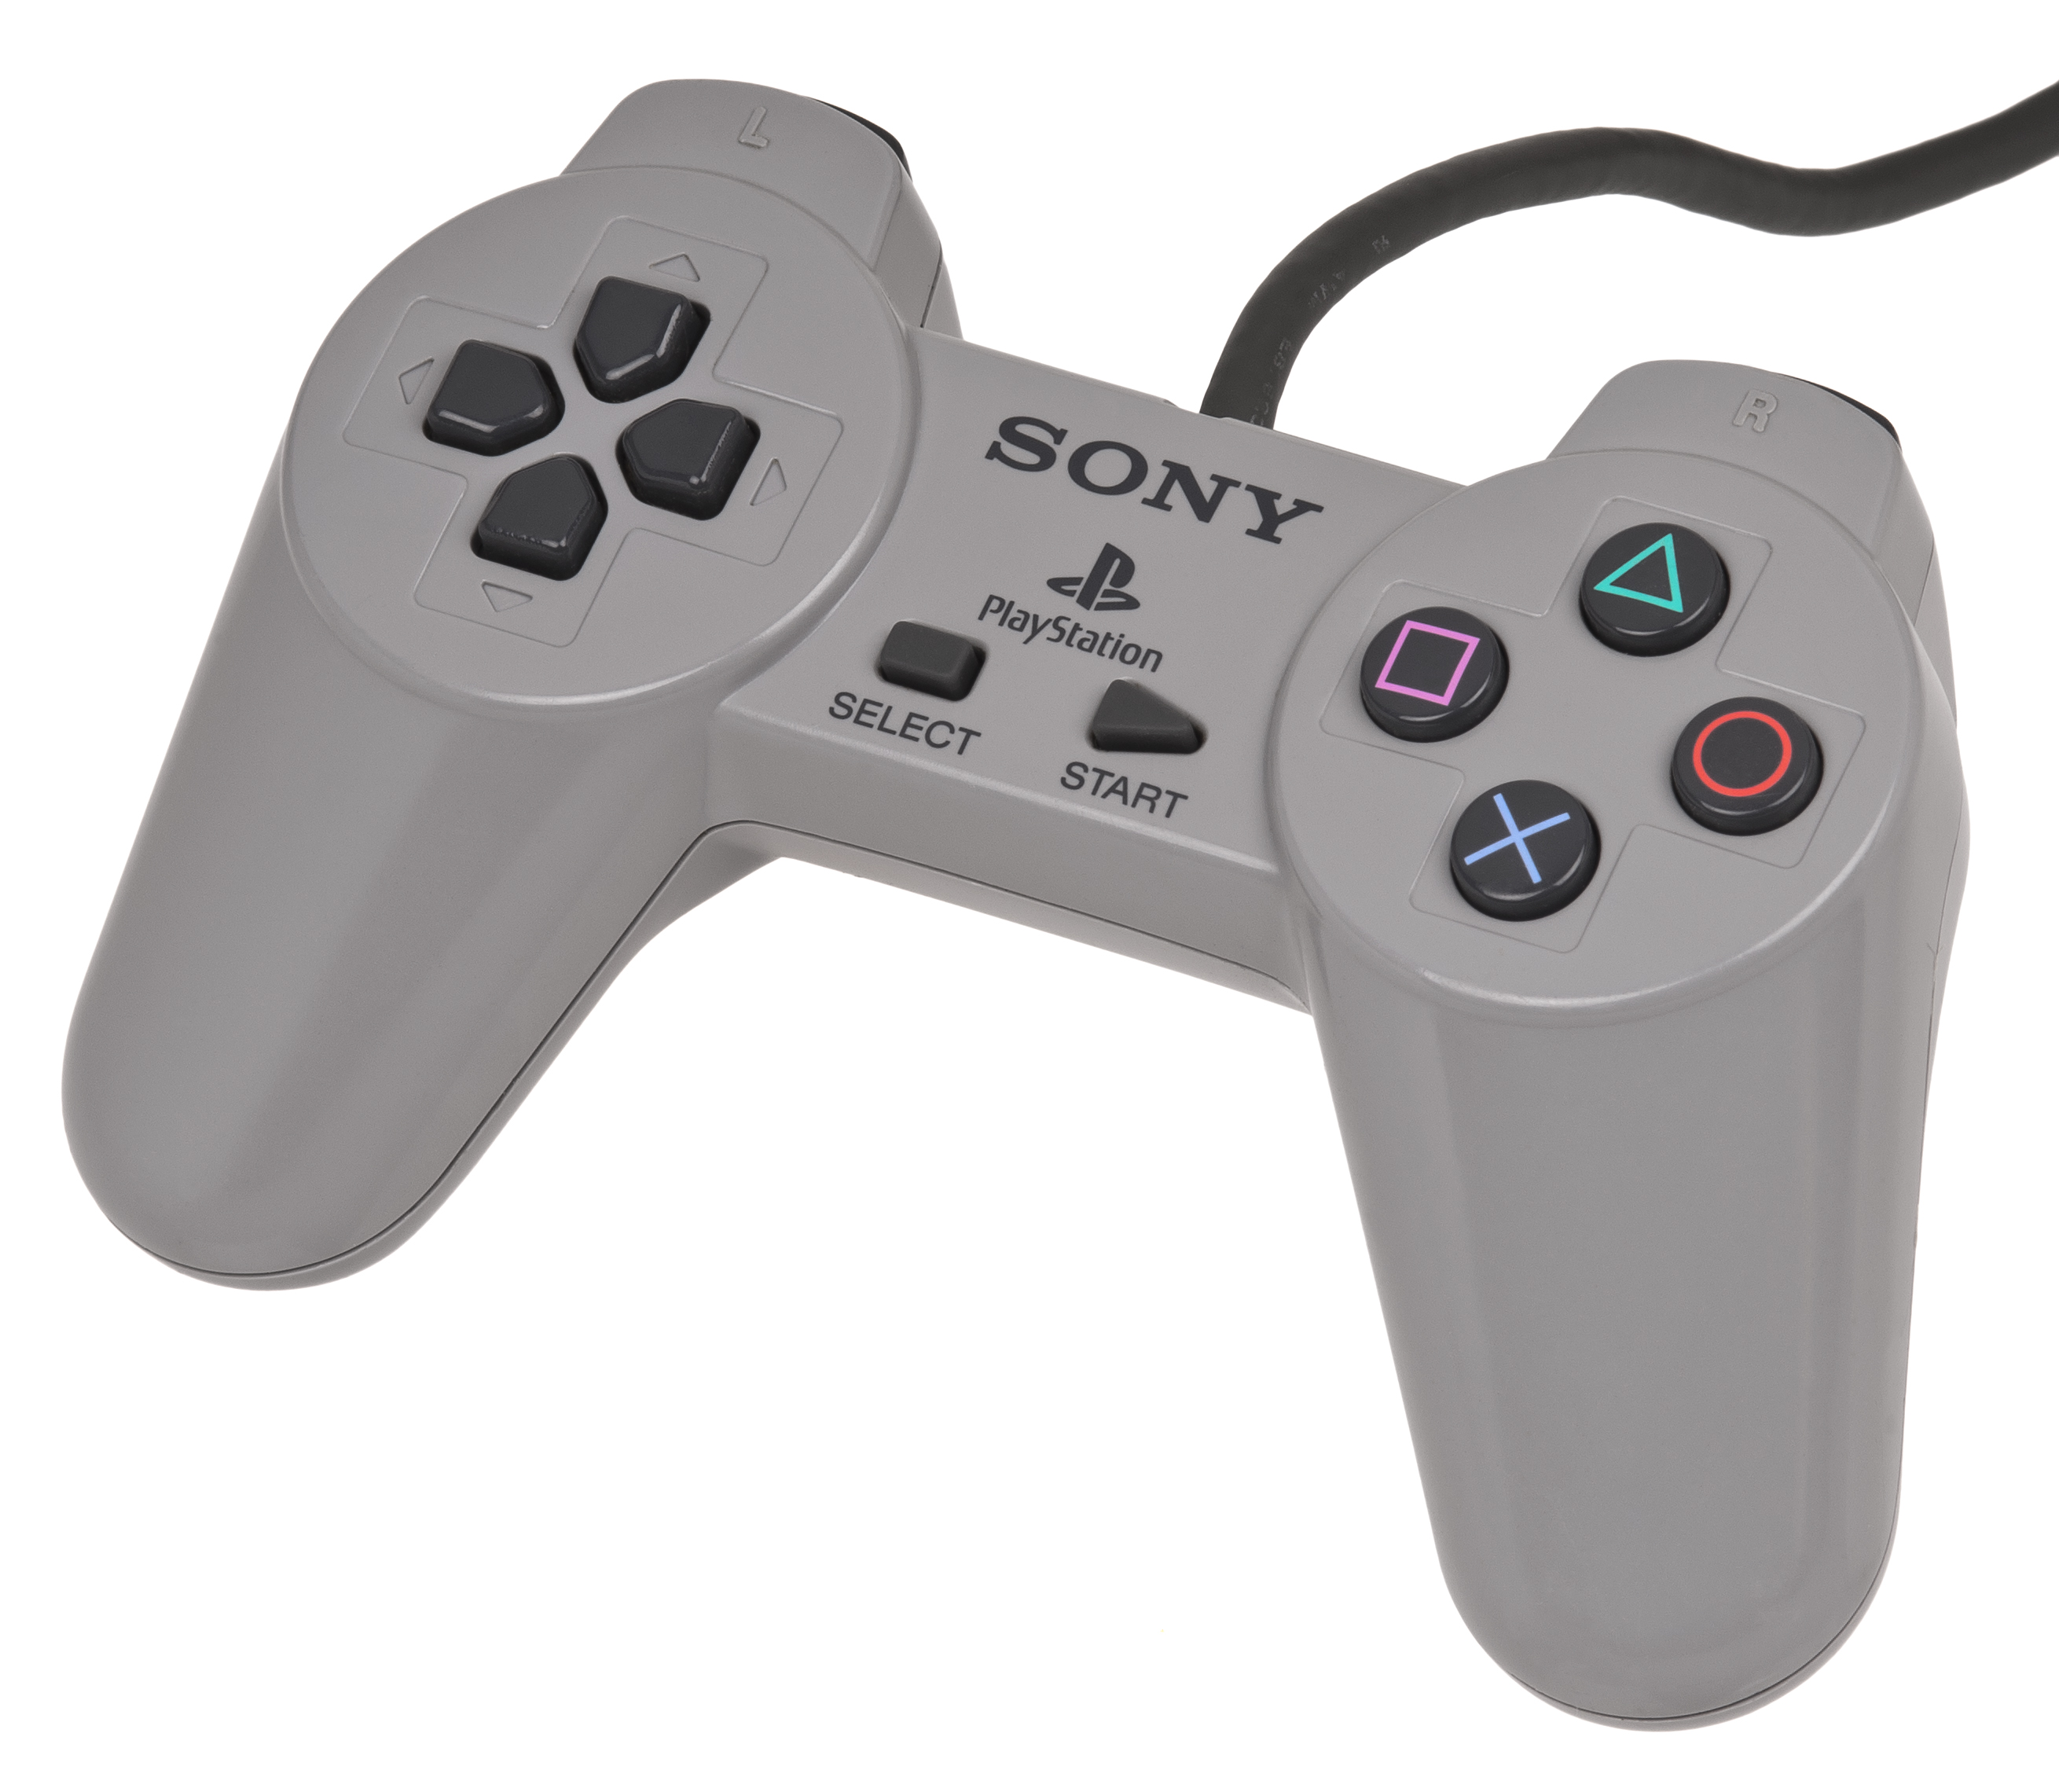
\includegraphics[width=0.3\textwidth]{ps_controller}
    }
    \subfloat[Steering Wheel Controller\label{fig:wheel}]{
      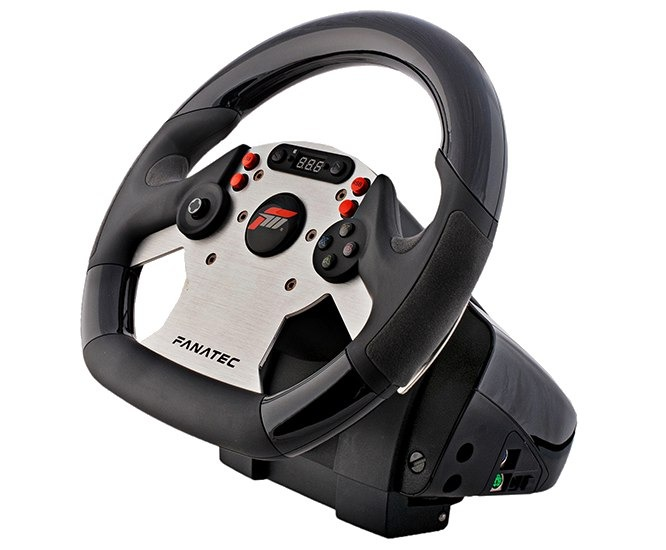
\includegraphics[width=0.3\textwidth]{steering_wheel}
    }
    \subfloat[Joystick\label{fig:joystick}]{
      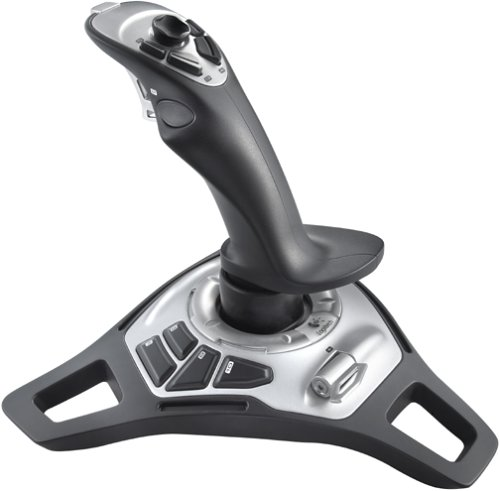
\includegraphics[width=0.3\textwidth]{logitech_joystick}
    }
    \caption{Examples of Input Devices for Gaming}
\end{figure}



\subsection{Mobile User Interfaces}

Very soon, technological progress made it possible to stick microcomputers
virtually in any device, be it a fridge, microwave oven or a car. The most
benefit out of this, however, gained the industry of mobile phones, eventually
giving birth to the concept of smart-phones. Today, almost every person living
in a more or less civilized region of the world has in his/her pocket a little
'brick' with the computer power thousands of times greater than the one that
was used to send people to the moon. This breakthrough in portable computing
facilitated the development of software for such devices and the majority of
companies started to support mobile applications where it made sense.

In the context of user interface design and input handling techniques,
developers found themselves in a completely different world. Nobody would
carry a mouse and a keyboard in order to interact with the phone, instead,
people would use the number pad plus a couple of additional buttons present on
the phone. In time, another revolution took place, it was the moment when
touch screens became reality. Once again, developers had to think their way
through these changes and create user interfaces that would suit fingers
poking into the screen rather than button clicks. With the difficulties of
user interface redesign for touch devices came also a wide range of new
possibilities. Now that the whole screen constituted an input device, the
users could perform gestures like taps, swipes, pan motions, pinch-zoom
actions. These gestures made the process of using an application a great deal
more intuitive when compared to the times when every action was performed
through the click of a certain button.

Besides touch screens, mobile phone vendors began to include in their devices
such sensors like accelerometers and gyroscopes. Accelerometers are used to
catch the moment when the device is moved and to calculate the direction and
acceleration of such movement. On the software side this could be used in
various ways, the simplest being to switch to the next song in the music
player by jerking the phone to the right. Meanwhile, gyroscopes where designed
to capture the orientation of the device at a given moment in time. This
functionality is employed every time the phone is tilted over 90 degrees and
triggers the switch between landscape and portrait view modes.

\newpage

When it came to the industry of mobile gaming, touch screens and sensors that
could capture the motion and orientation of the device were a really big deal,
because they opened the possibilities for developing complex user interfaces
that would simulate specialized gaming devices. The accelerometer and
gyroscope would be used as the steering wheel in racing games while the touch
screen would capture taps in various regions and interpret them as clicks of
different buttons of a gamepad, whose simplified image would be rendered on
the same screen.

% picture of mobile game UI which resembles a gamepad

\subsection{Mobile Devices as Controllers for Desktop Computers}

When comparing the features of a specialized gaming device like \emph{Nintendo
Wii}\cite{wiimote} Controller and the capabilities of a modern smart-phone, an interesting
pattern of similarities can be observed. Both are able to capture device
motion and position. Both respond to clicks of buttons in case of a gamepad
and taps in designated areas in case of a phone. Touch screens can be used to
simulate even the motion of a joystick, by capturing swipe or pan gestures.
One feature that a specialized gaming device may have, that a phone falls
short of, is ergonomics, but to a certain extent this can be neglected. With
such a list of similarities, a logical question appears: Why not use mobile
phones as gaming controllers for desktop games?


\subsubsection{Usability Limitations}

As it turns out, now that smart-phones run full-fledged operating systems,
connecting one to a computer is not that hard of a task. Mobile operating
systems like Android, Apple iOS and Windows Mobile, all support socket
programming, thus a programmer can setup a communication channel over the
network between a mobile phone and a laptop connected to the same Wi-Fi
hotspot. They can even be located on different sides of the planet, it is
sufficient to have an Internet connection to be able to exchange data between
devices.

Overall it looks like a way to go approach. On the other hand, there are some
problems with it that are not to be observed at first sight. In the first
place, every time that a company wants to create a game with support for
mobile devices as controllers, the developers will have to write custom mobile
applications in addition to the main game, they will also have to devise
specialized communication protocols. This is both, time and money consuming
and is not economically convenient. Secondly, there is a problem on the user
side which is best illustrated with a situation. Let's suppose a party or a
team-building event where the host tries to entertain his guests with a
multiplayer computer game. Not everyone has at home a gaming platform like
Sony Playstation or Microsoft Xbox, neither does anyone have more than 2-3 PC
gamepads. In this situation, the ability to use smart-phones as controllers
would be a great benefit. In case the connection is implemented in the way
described above, a gaming party would transform into a setup party, where
guests would spend a lot of time installing mobile applications that are
probably needed only for one-time use and don't hold any value by themselves
without the main game. Fortunately both problems can be solved relatively
simple through the same solution.

\newpage

\subsubsection{Web-based Workaround}

One thing that all modern smart-phones have in common is a decent web browser.
Today, browsers are more than just viewers of HTML documents, they are entire
ecosystems and programming environments that are almost independent of the
underlying operating system. The fact that every mobile phone has such an
environment makes it possible to write cross-platform application served on
the web that would otherwise be installed manually as a native app. Modern
browsers support APIs that can interact with various parts of a mobile device
like accelerometer, gyroscope and touch screen, exactly the things that are
necessary to simulate a fully functional gaming device.

Having said this, one thing that could solve the problems stated in the
section above may be a framework or toolkit that unifies in a single library
all the APIs that are necessary to connect a mobile phone to a computer as a
remote gaming controller. It would make it easier and faster to develop games
with such a feature. This toolkit may also include user interface building
blocks which can be combined to create custom controllers.

The purpose of this thesis is to create a simple web-based multiplayer
isometric arcade called 'Snowfight'. The main game is started by accessing its
web page. The first thing the players see is a lobby and a connection URL.
Players join the game by navigating to the provided URL using the browsers
installed on their phones. When enough players have connected and the
participants decide to start the game, a button can be clicked on the main
game screen. The game play concept is rather simple, players can move their
characters around the game space and throw snowballs in each other using the
controls rendered by the web application that works on their phones. Every
player has a certain amount of hit points (HP) and if a player is hit, his HP
amount decreases. When a player's HP amount reaches zero, he is eliminated
from the game. The goal of the game is to eliminate all players from the
adversary team.

In order to implement this project it is necessary to explore the topic of
real-time communication in the web, as to be able to chose the right technology
that would provide a smooth and responsive gaming experience.


\subsection{Real-Time Communication over the Web}

One of the main uses of the Internet is hosting and accessing web pages. When a
user writes a URL in the browser's search bar and presses 'enter', the browser
preforms an HTTP request to the server specified by the URL and fetches a web
page. At this point in time, for most cases, the communication between the
server and the client (browser) is ceased until the user clicks on another link
that would restart the process.

On the other hand, modern web has greatly developed during the past few years.
Internet connection speed has increased dramatically, and many websites have
stopped being just static web pages and have moved towards a more dynamic model.
They are not even called websites, today, all around the world there are web
applications.

With the requirements for a more dynamic web came also the technical challenges
of making it so. For instance, how would a user's browser receive a notification
about a message that was sent to this user from another part of the globe? When
such questions just appeared, developers tried different techniques using the
old tools they had at hand at that time. The concepts of HTTP Long Polling and
HTTP Streaming appeared in this period. Soon, however, they were found to be
causing quite a bit of issues\cite{long_polling_issues} and a need for custom
protocols arose.

As the web is mainly composed of clients and servers, the logical outcome was a
protocol that would connect them and would permit bidirectional communication
between the server and its clients, thus WebSockets were proposed. At the same
time, browsers grew and their uses extended. Soon, real-time communication out-
sized the context of client-server architecture and when video chat applications
and multiplayer games started to conquer the web realm, engineers developed
WebRTC, which solved the issue of communication in peer-to-peer setups. A brief
description of both protocols as per their RFCs is presented in the sections
that follow.

\subsubsection{WebSockets for Client-Server Communication} % Websockets

Historically, creating web applications that need bidirectional communication
between a client and a server (e.g., instant messaging and gaming applications)
has required an abuse of HTTP to poll the server for updates while sending
upstream notifications as distinct HTTP calls.

As RFC6455\cite{websockets} points out, this results in a variety of problems:

\begin{itemize}

\item The server is forced to use a number of different underlying TCP
  connections for each client: one for sending information to the
  client and a new one for each incoming message.

\item The wire protocol has a high overhead, with each client-to-server
  message having an HTTP header.

\item The client-side script is forced to maintain a mapping from the
  outgoing connections to the incoming connection to track replies.

\end{itemize}

A simpler solution would be to use a single TCP connection for traffic in both
directions. This is what the WebSocket Protocol provides. Combined with the
WebSocket API, it provides an alternative to HTTP polling for two-way
communication from a web page to a remote server.

The same technique can be used for a variety of web applications: games, stock
tickers, multiuser applications with simultaneous editing, user interfaces
exposing server-side services in real time, etc.

The WebSocket Protocol is designed to supersede existing bidirectional
communication technologies that use HTTP as a transport layer to benefit from
existing infrastructure (proxies, filtering, authentication). Such technologies
were implemented as trade-offs between efficiency and reliability because HTTP
was not initially meant to be used for bidirectional communication. The
WebSocket Protocol attempts to address the goals of existing bidirectional HTTP
technologies in the context of the existing HTTP infrastructure; as such, it is
designed to work over HTTP ports 80 and 443 as well as to support HTTP proxies
and intermediaries, even if this implies some complexity specific to the current
environment. However, the design does not limit WebSocket to HTTP, and future
implementations could use a simpler handshake over a dedicated port without
reinventing the entire protocol. This last point is important because the
traffic patterns of interactive messaging do not closely match standard HTTP
traffic and can induce unusual loads on some components.

\newpage

\subsubsection{WebRTC for Peer to Peer Communication} % WebRTC

Real-time communication has been on the market for a while, however, it was
implemented mainly in corporate environments as in-house solutions. It was quite
expensive in terms of effort to include such technology in existing projects
especially in the context of the web. In recent years this started to change
with the appearance of various frameworks and APIs.

WebRTC\cite{webrtc_org} is a free, open project that provides browsers and
mobile applications with Real-Time Communications (RTC) capabilities via simple
APIs. The WebRTC components have been optimized to best serve this purpose.
Due to its properties, WebRTC is of particular interest for the development
of the project for the present thesis.

As Sam Dutton points out in his article\cite{webrtc_basics}, WebRTC has now
implemented open standards for real-time, plugin-free video, audio and data
communication. This solves a range of problems relevant to real-time
communications:

\begin{itemize}
    \item Many web services already use RTC, but need downloads, native apps or
        plugins. These includes Skype, Facebook and Google Hangouts.

    \item Downloading, installing and updating plug-ins can be complex, error
        prone and annoying.

    \item Plugins can be difficult to deploy, debug, troubleshoot, test and
        maintain, and may require licensing and integration with complex,
        expensive technology. It's often difficult to persuade people to install
        plugins in the first place.
\end{itemize}

The guiding principles of the WebRTC project are that its APIs should be open
source, free, standardized, built into web browsers and more efficient than
existing technologies. Presently it is capable of enabling efficient
transmission of audio, video and arbitrary data in a peer-to-peer fashion. At
the same time WebRTC still needs servers because of the following
reasons\cite{webrtc_realworld}:

\begin{itemize}

\item For clients to exchange metadata to coordinate communication: this is
called signaling.

\item To cope with network address translators (NATs) and firewalls.

\end{itemize}



\begin{figure}[!h]
\centering
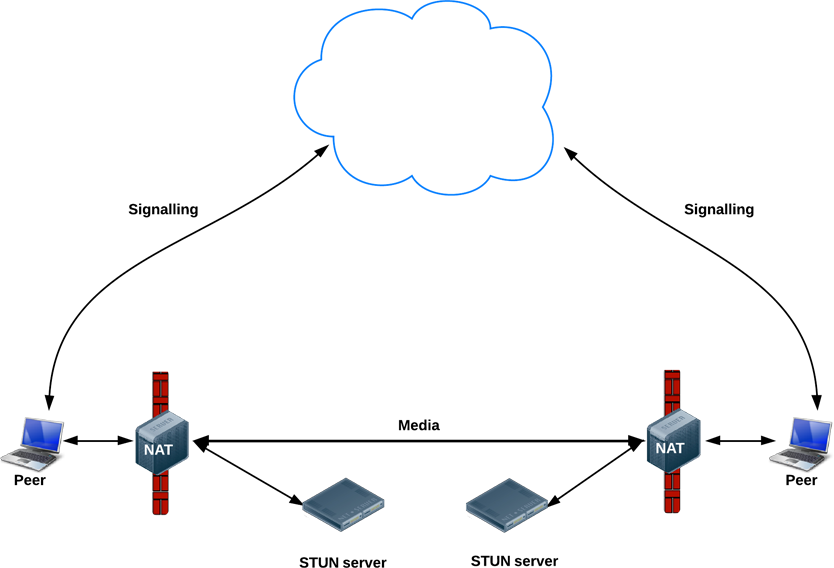
\includegraphics[width=12cm]{webrtc_stun}
\caption{Session Traversal Utilities for NAT (STUN)}\label{fig:stun}
\end{figure}

Signaling is the process of coordinating communication. In order for a WebRTC
application to set up a 'call', its clients need to exchange information like
session control messages, error messages, as well as metadata and settings. This
signaling process needs a way for clients to pass messages back and forth. To
avoid redundancy and to maximize compatibility with established technologies,
signaling methods and protocols are not specified by WebRTC standards. This
approach is outlined by the JavaScript Session Establishment
Protocol\cite{jsep}.

In order to find the best route from peer to peer, WebRTC makes use of ICE
(Interactive Connectivity Establishment) technologies. Usually two kinds of
methods are used, Session Traversal Utilities for NAT (STUN) and Traversal Using
Relays around NAT (TURN). WebRTC uses a STUN server to find a direct connection
between peers in order to achieve the smallest latency. If no such connection
can be established, the process falls back to using a TURN server that works as
relay for all further communications. Figures \ref{fig:stun} and \ref{fig:turn}
showcase both situation in a visual manner:

\begin{figure}[!h]
\centering
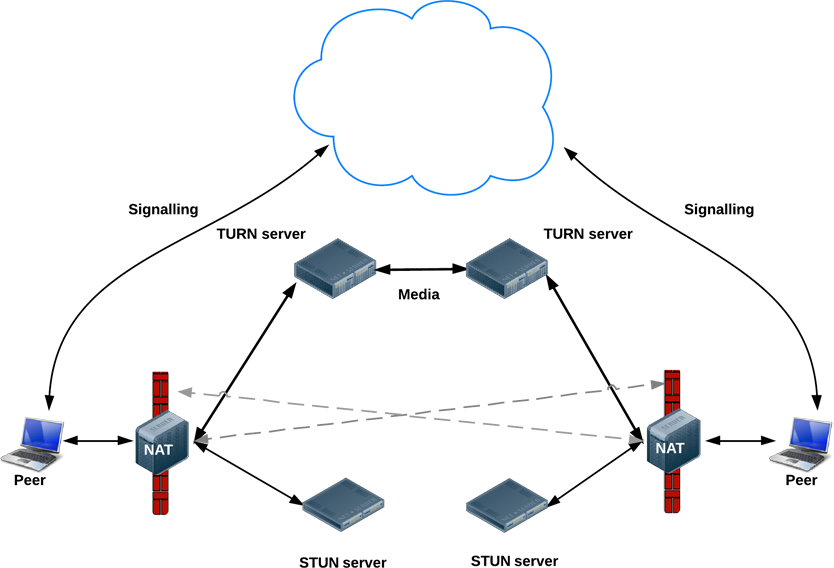
\includegraphics[width=12cm]{webrtc_turn}
\caption{Traversal Using Relays around NAT (TURN)}\label{fig:turn}
\end{figure}

WebRTC is the most appealing technical solution for the project proposed in this
thesis. The protocol will make sure that the players will be connected to the
game using the shortest possible network route therefore having the smallest
latency. In most cases players will be located behind the same NAT, and after
establishing a connection, no data will travel further than to the router.


% \subsection{Mobile devices Game Controllers} % game controllers + web

% \subsubsection{Native Apps}

% \subsubsection{Web Apps}

\subsection{Existing Solutions on the Market}

Even though WebRTC is a quite fresh technology, there are already plenty of
projects using it. Some of these projects are created by developers as part of
the Chrome Experiments\cite{chromeexperiments} project, in order to demonstrate
the technology and its capabilities. Two projects in particular are of interest
to this thesis as they represent the concept of a mobile phone being used as a
gaming controller. The following sections briefly describe the games and point
out things that may be applied to this thesis.

\subsubsection{Lightsaber Escape} % https://lightsaber.withgoogle.com/

The Lightsaber Escape\cite{lightsaber} is a small single-player arcade game
created by Lucasfilm Ltd in collaboration with Google in order to promote the
seventh film in the Star Wars trilogy. It requires a personal computer a
supported mobile device and an Internet connection. To play the game, the user
has to access the main page of the game
(\url{https://lightsaber.withgoogle.com/}) in a browser window on the computer
(figure \ref{fig:lightsaber_home}).

\begin{figure}[!h]
\centering
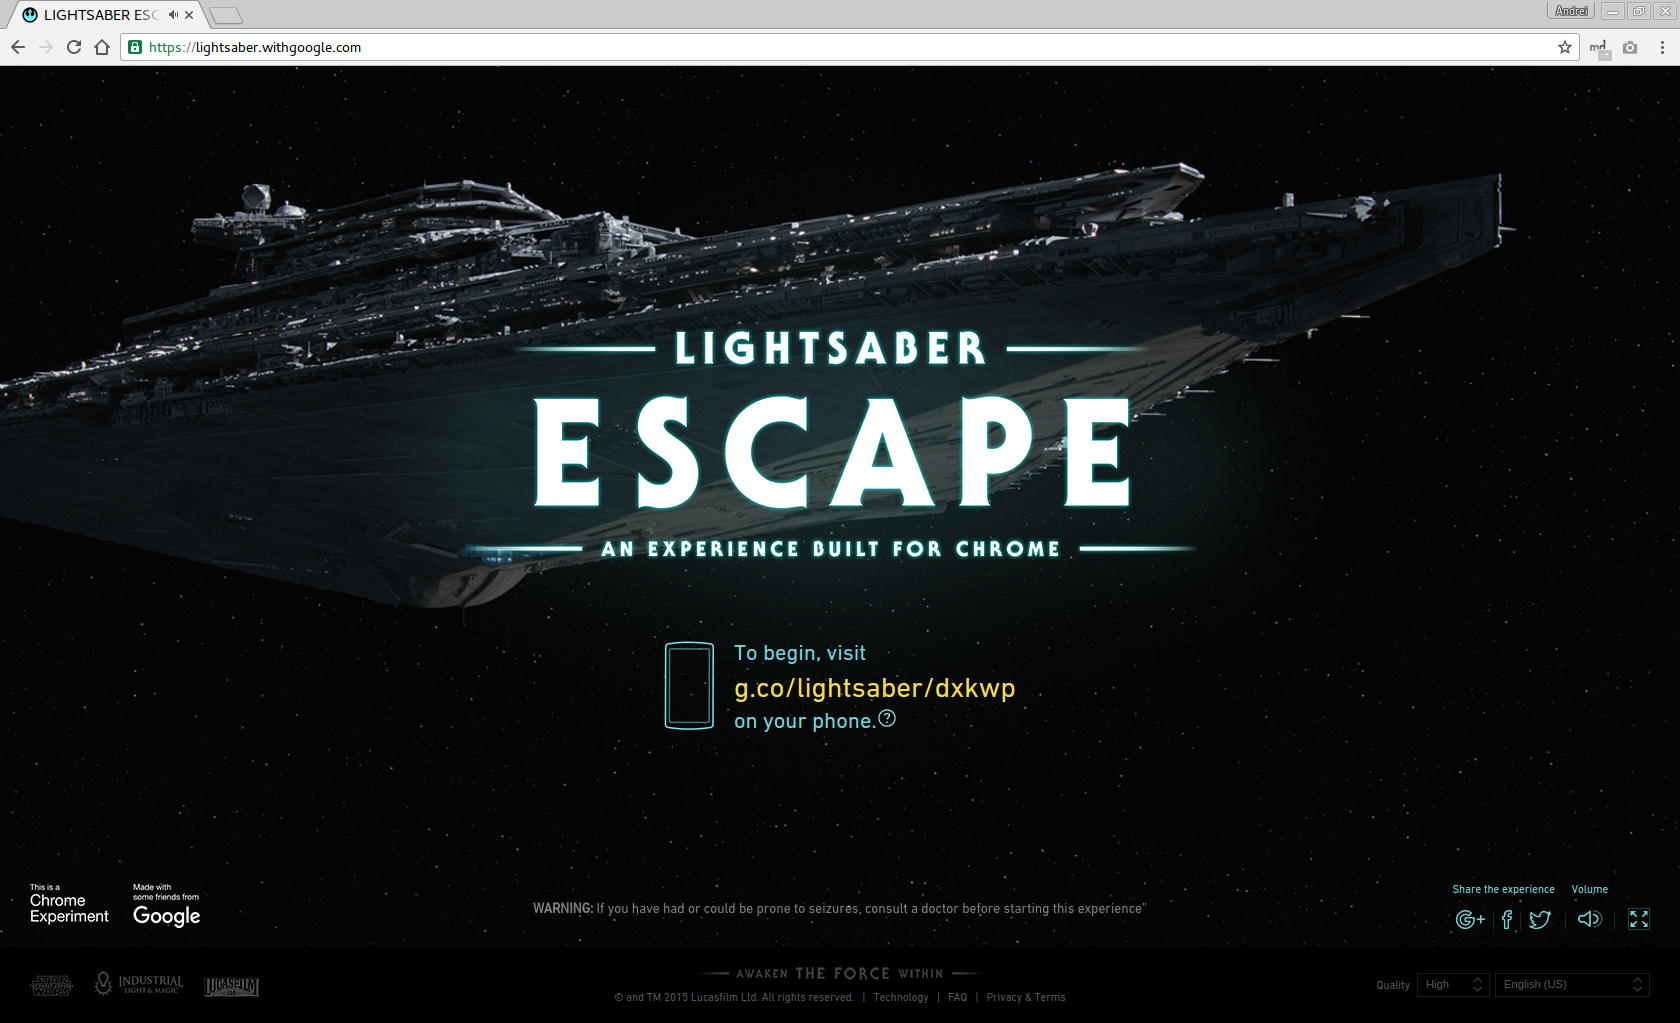
\includegraphics[width=10cm]{lightsaber_home}
\caption{Home Page of Lightsaber Escape}\label{fig:lightsaber_home}
\end{figure}

The user is presented with a short link that has to be entered in the navigation
bar of the browser on the mobile device. This brings the user to a page with
instructions to calibrate the device (figure \ref{fig:lightsaber_calibrate}).
During the calibration process, a connection is established between the phone
and the computer and the phone's gyroscope and accelerometer are calibrated.
After this procedure the lightsaber becomes active (figure
\ref{fig:lightsaber_active}):

\begin{figure}[!ht]
    \centering
    \subfloat[Calibration Screen\label{fig:lightsaber_calibrate}]{
      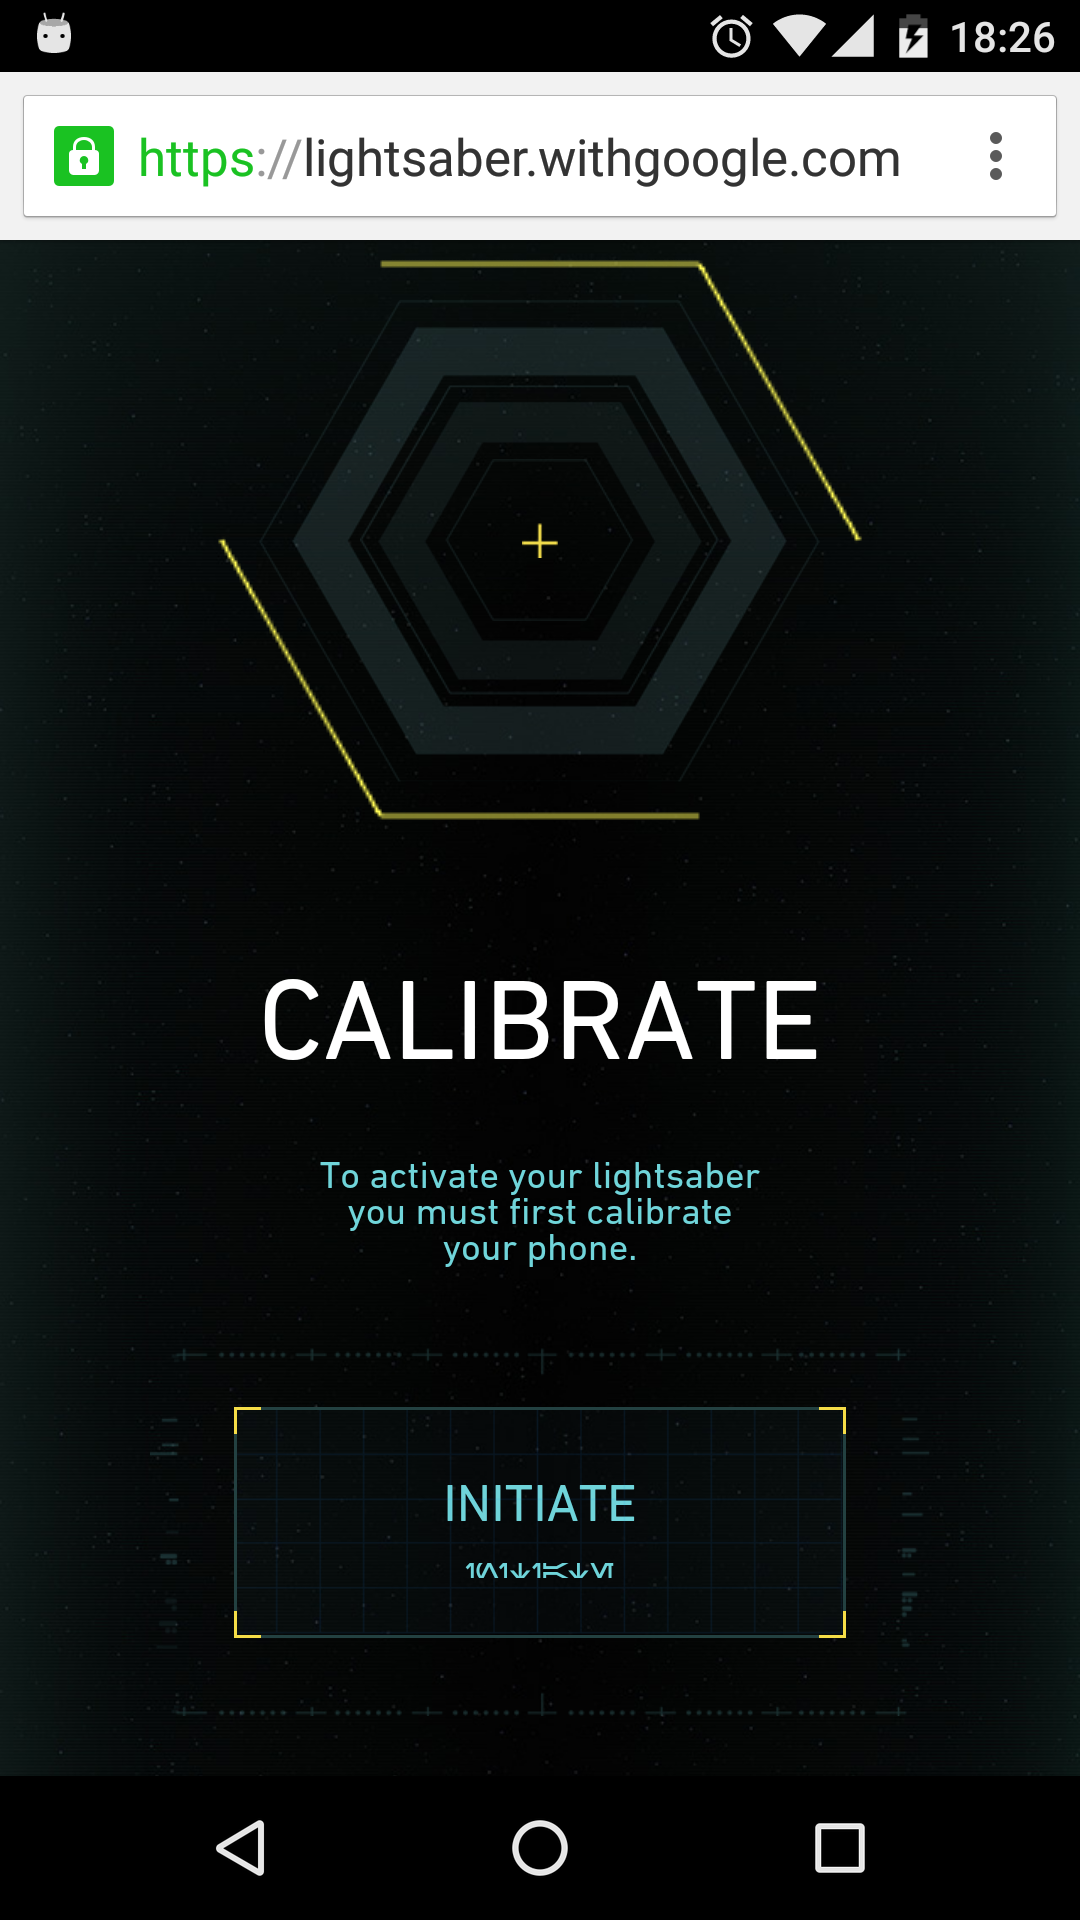
\includegraphics[width=0.25\textwidth]{lightsaber_calibrate}
    }
    \hspace{0.1\textwidth}
    \subfloat[Active Lightsaber\label{fig:lightsaber_active}]{
      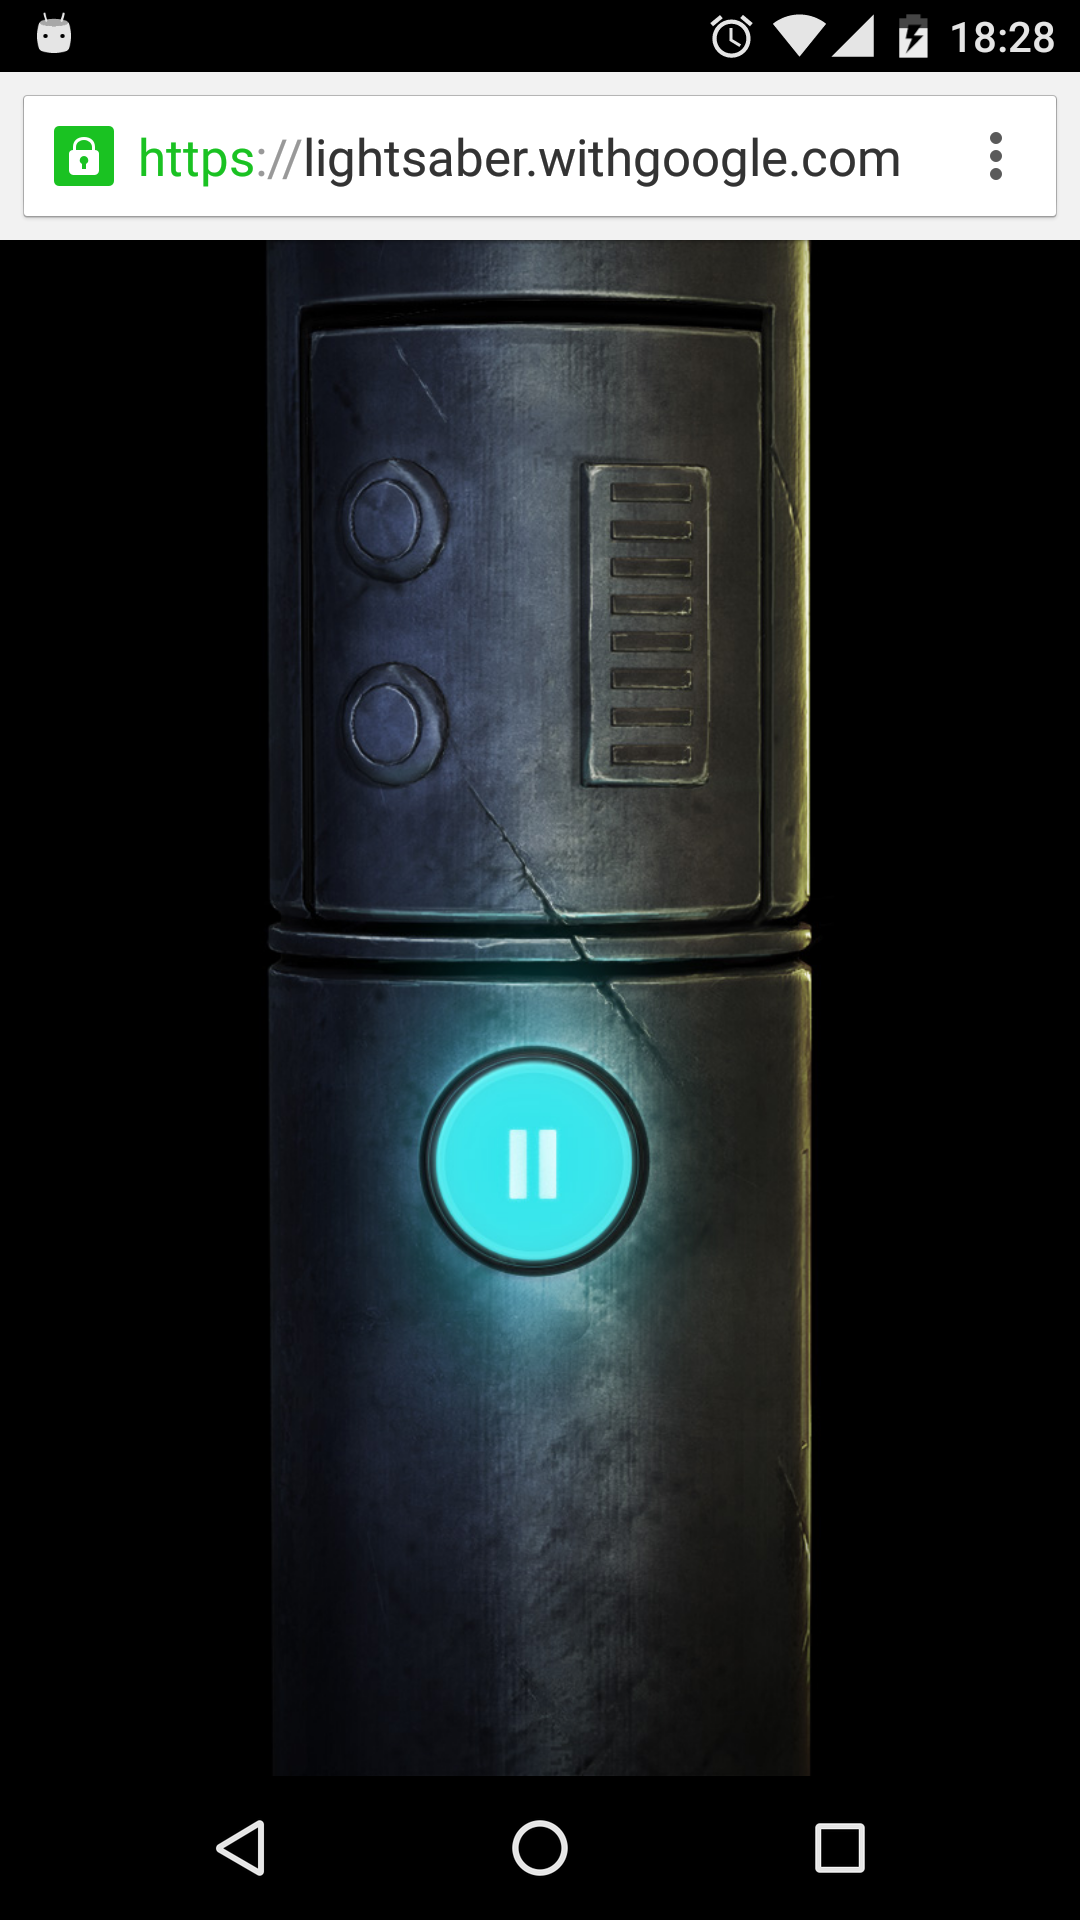
\includegraphics[width=0.25\textwidth]{lightsaber_active}
    }
    \caption{Lightsaber Escape as Seen on a Mobile Phone}
\end{figure}

With an active lightsaber, the player can start the gameplay, which consists of
dodging enemy laser blasts by controlling the lightsaber through movements of
the mobile phone. The player passes a couple of corridors in such a manner,
until he/she reaches a hand-to-hand combat encounter that resolves to the game's
finale.

\begin{figure}[!h]
\centering
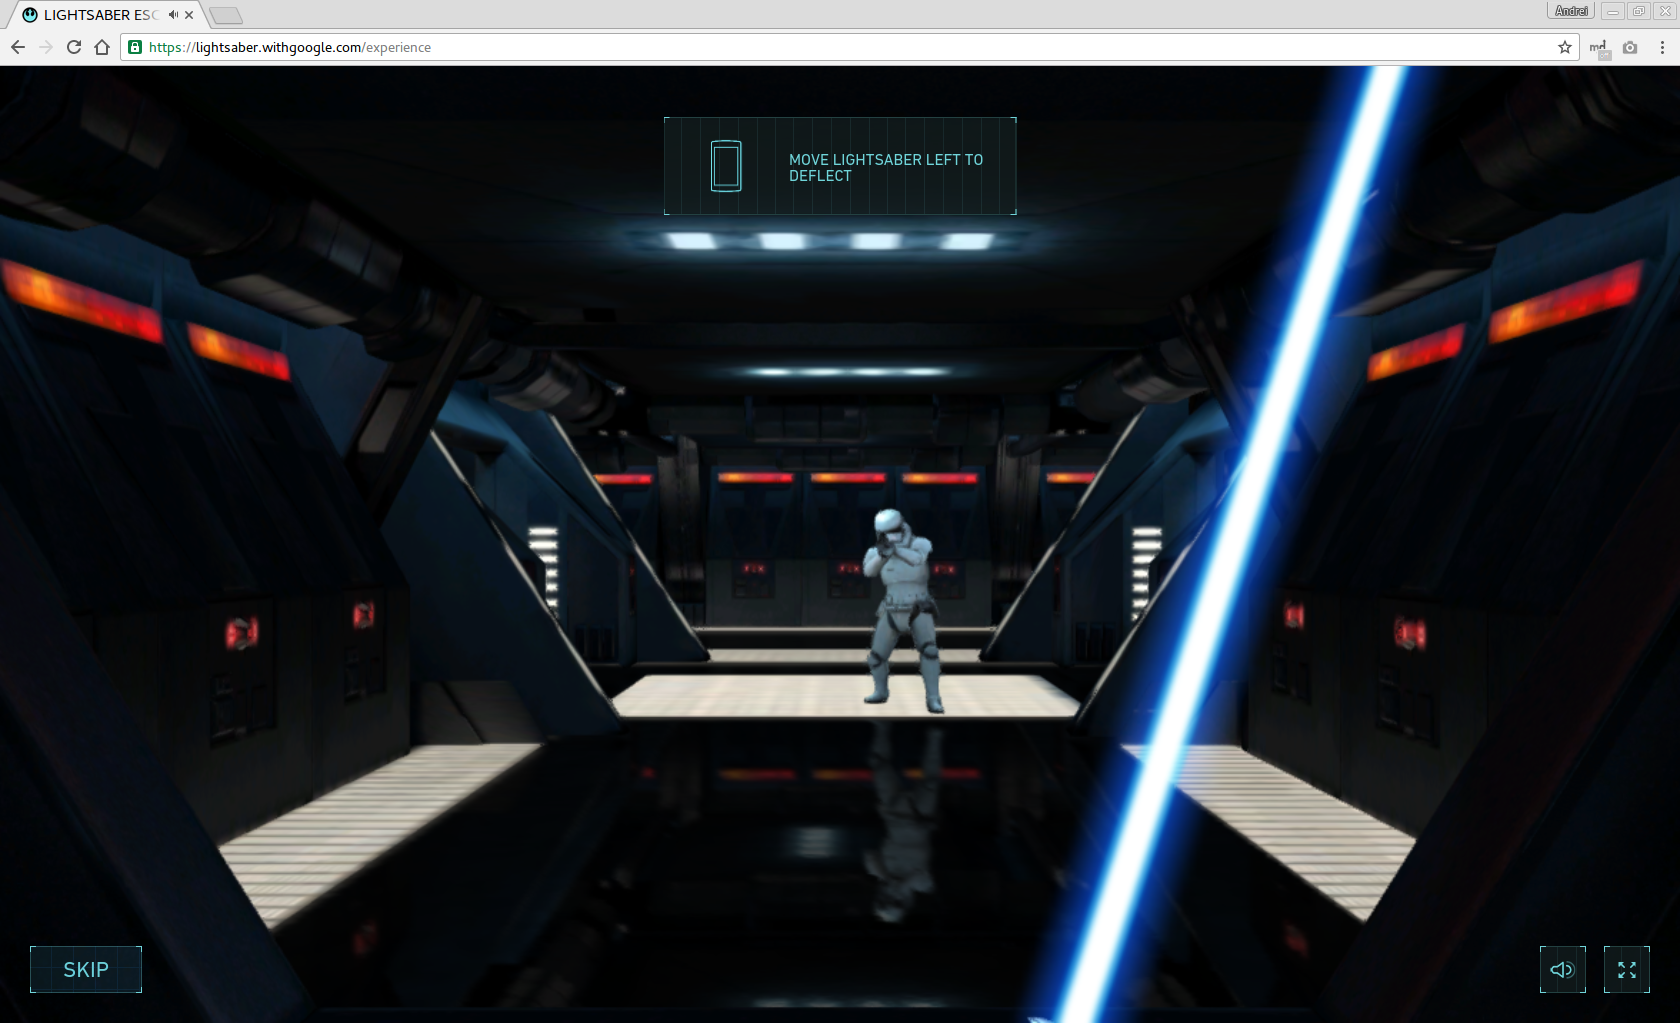
\includegraphics[width=10cm]{lightsaber_game}
\caption{Lightsaber Escape Gameplay}\label{fig:lightsaber_game}
\end{figure}

There are a couple of important things to note about this game. The clever way
in which are leveraged the motion-detection capabilities of a phone makes for a
really engaging experience, even though the whole gameplay lasts only about 5
minutes. If played on a powerful computer with a decent GPU, it could be noticed
that control mechanism is very smooth and responsive, this is thanks to an
efficient use of network traffic in the communication between devices. Overall
this game is a good way to promote a product using innovative technology and it
gives some hints on how to develop the project of this thesis.

\subsubsection{Super Sync Sports} % https://www.chrome.com/supersyncsports/

Super Sync Sports\cite{sports} is another Chrome Experiment with the same
concept of connecting a mobile phone to a computer in order to achieve an
interactive experience. This game has support for multiplayer gameplay for each
of the three game modes. Cycling mode is shown in figure \ref{fig:sports_game}.

\begin{figure}[!h]
\centering
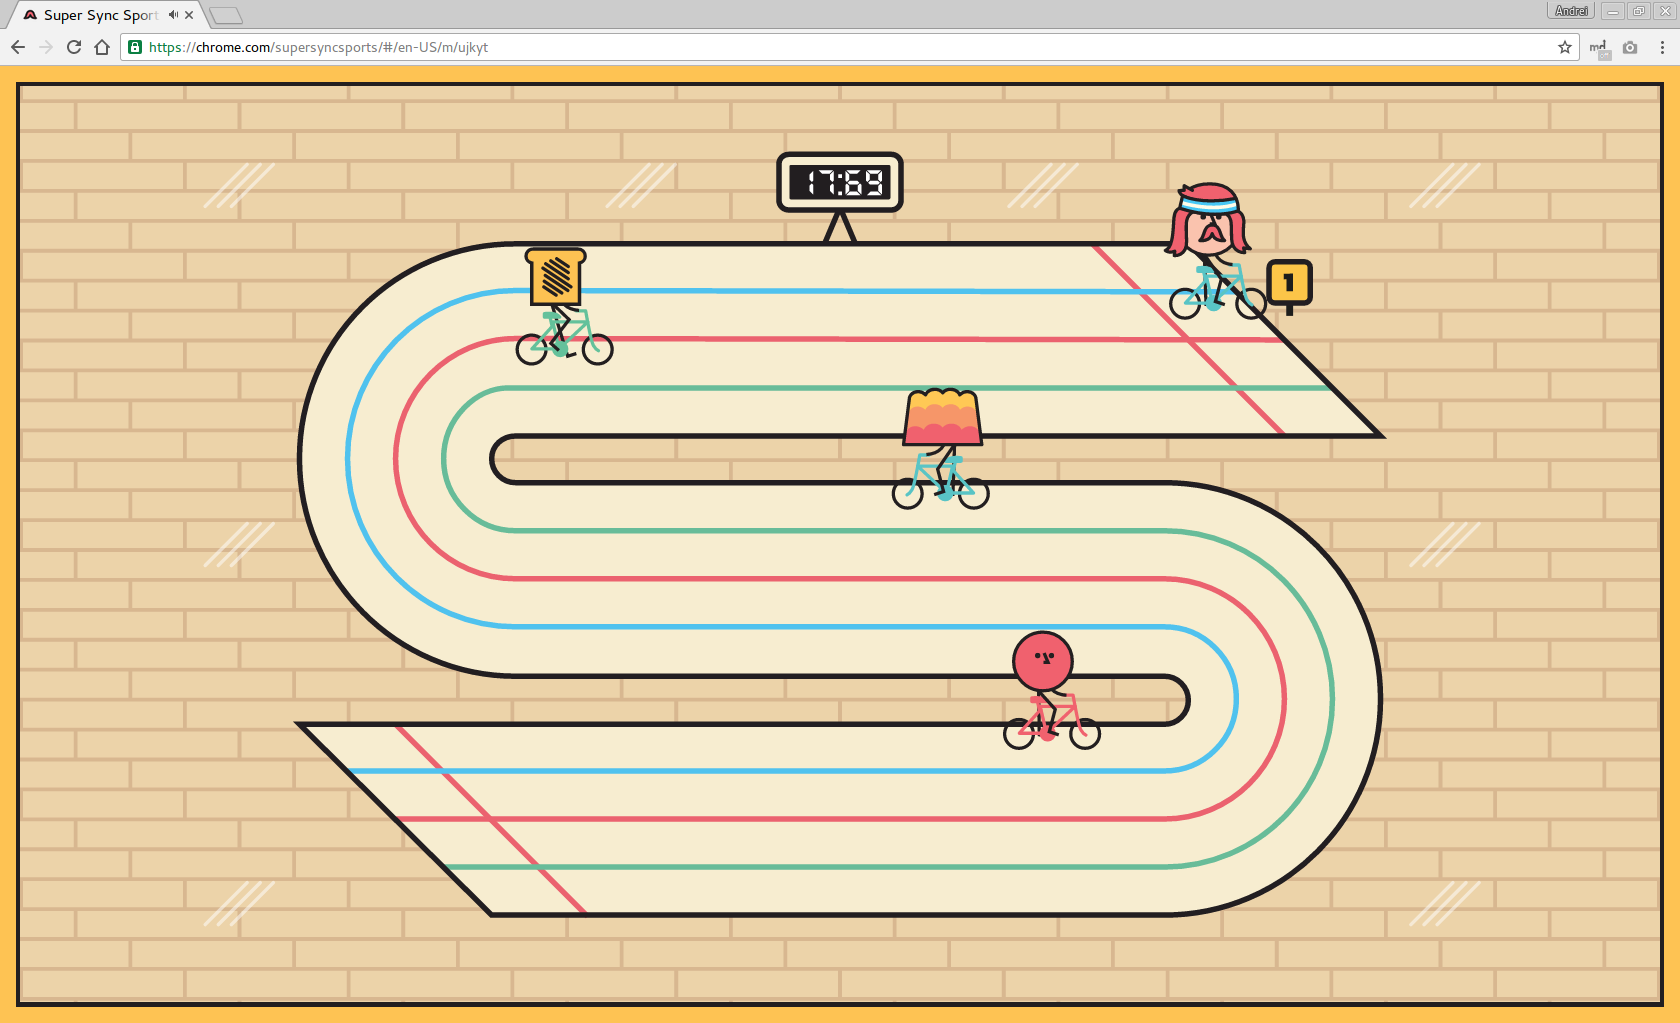
\includegraphics[width=10cm]{sports_game}
\caption{Super Sync Sports Cycling Challenge}\label{fig:sports_game}
\end{figure}

\newpage

Once connected, players can choose a character (figure \ref{fig:sports_player})
and use the controls on the phone (figure \ref{fig:sports_controls}) to race
with each other on a track. In contrast to Lightsaber Escape, does not use
motion-detection sensors of the phone, instead, the player activity is
controlled by sophisticated touch screen gestures.

\begin{figure}[!ht]
    \centering
    \subfloat[Character Selection Screen\label{fig:sports_player}]{
      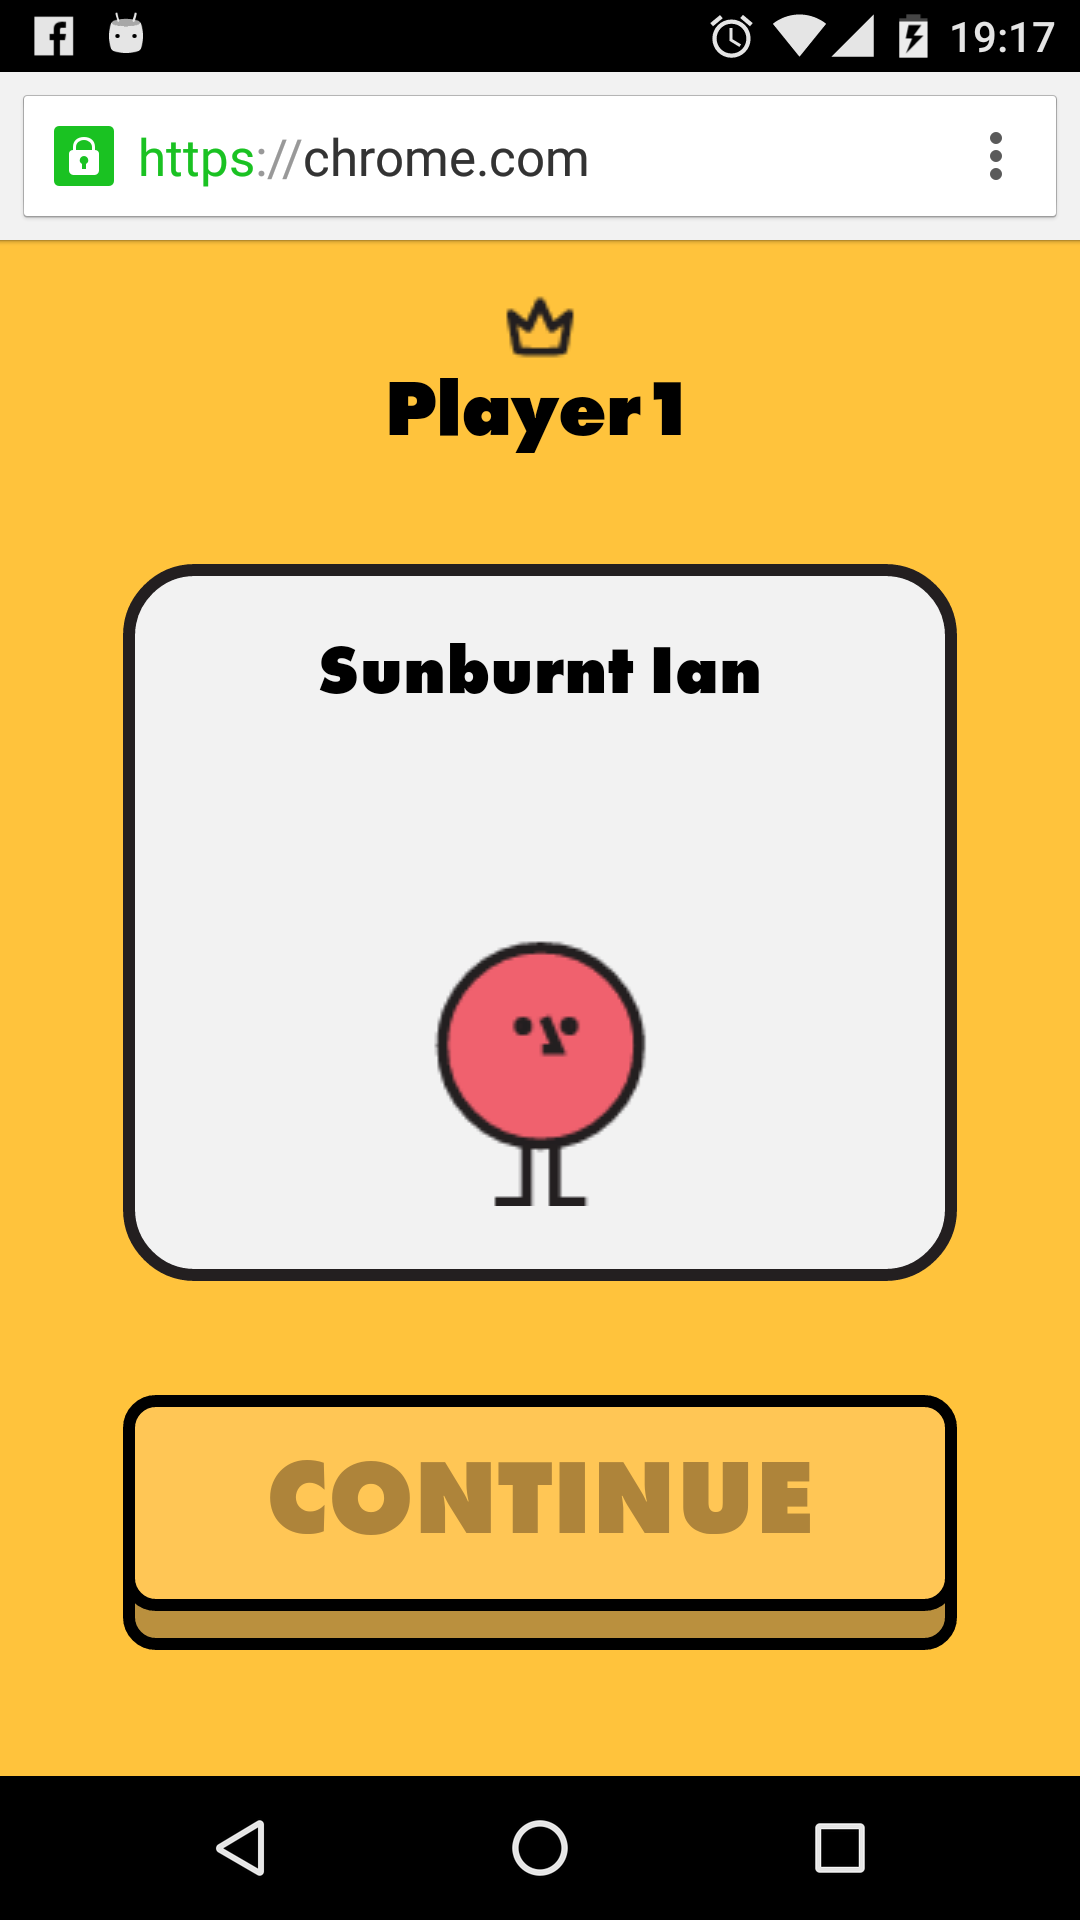
\includegraphics[width=0.25\textwidth]{sports_player}
    }
    \hspace{0.1\textwidth}
    \subfloat[Player Controls for Cycling Challenge\label{fig:sports_controls}]{
      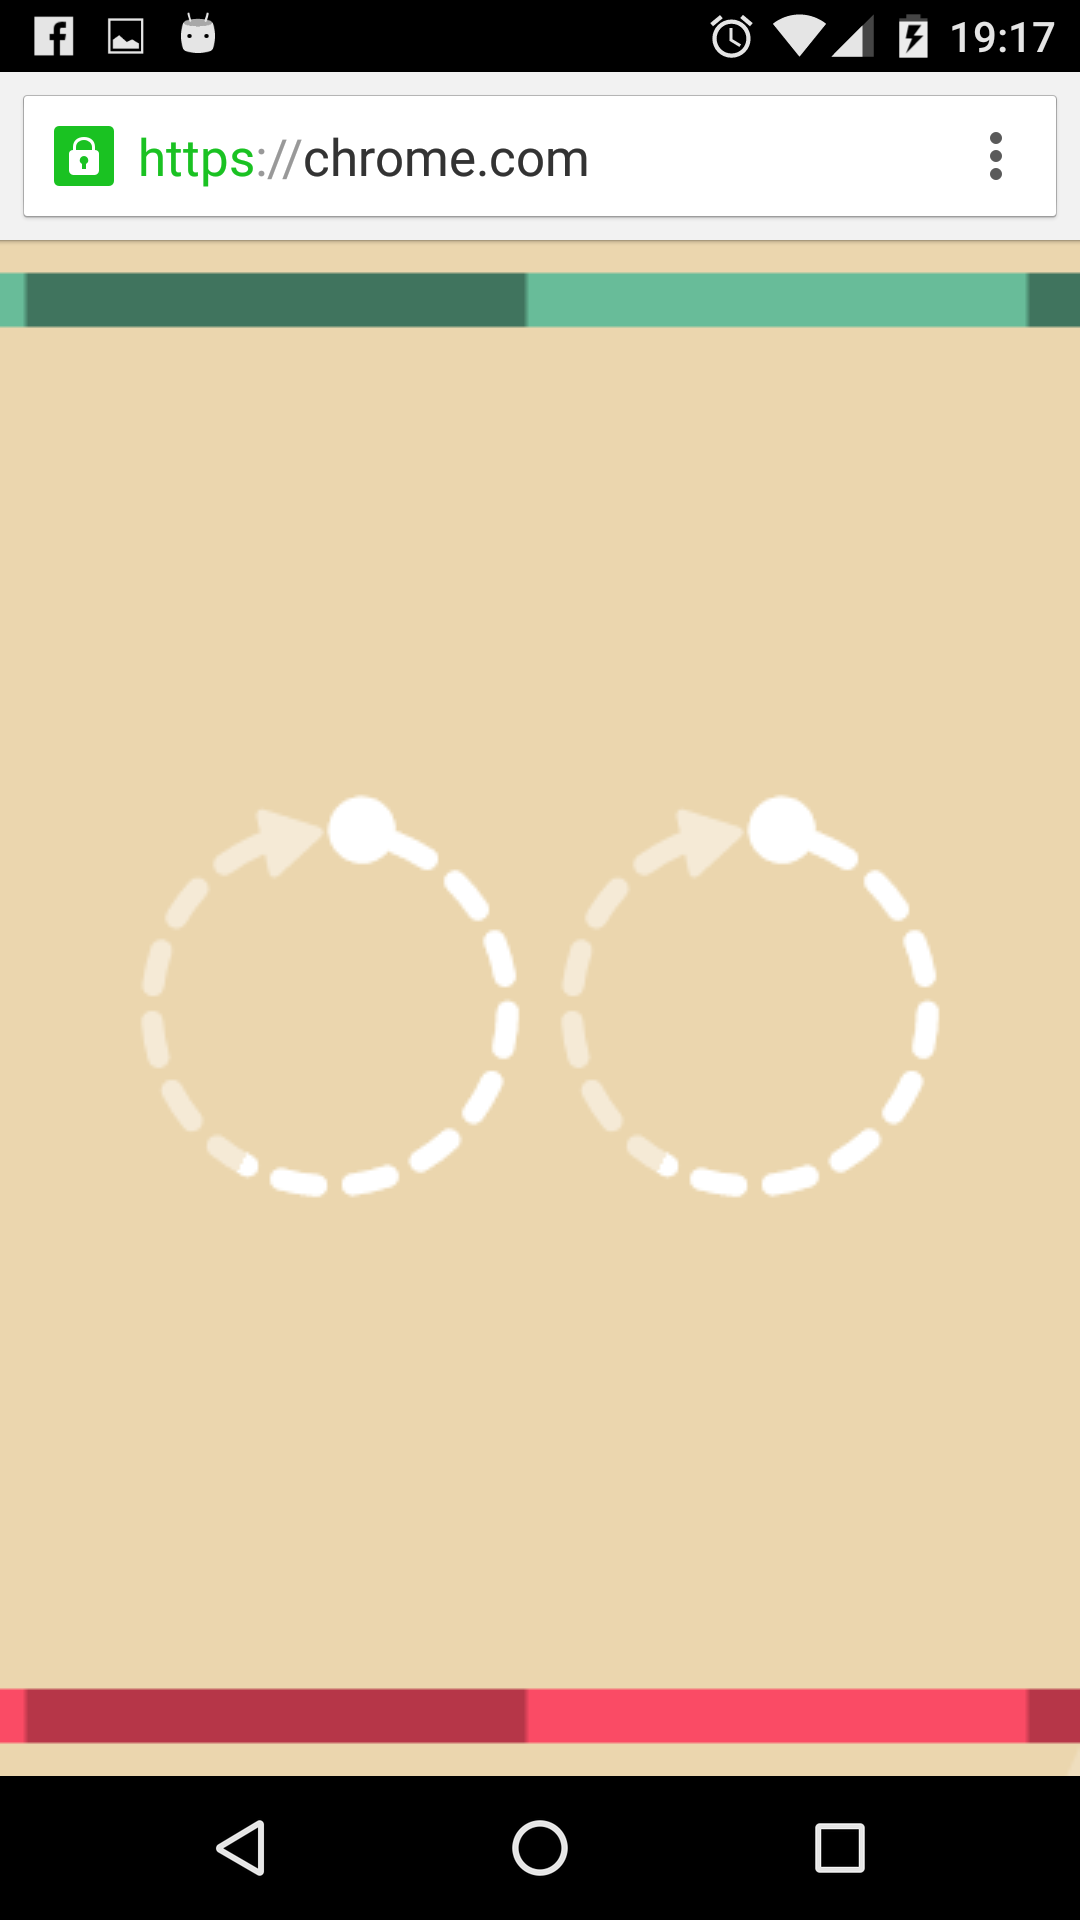
\includegraphics[width=0.25\textwidth]{sports_controls}
    }
    \caption{Super Sync Sports on a Mobile Phone}
\end{figure}

From the technical point of view, Super Sync Sports and Lightsaber Escape share
a lot of similarities like the connection procedures and the efficient use of
WebSockets technology. It is also interesting how Super Sync Sports delegates
things like character choice to the users phone rather than shows it on the
common game screen. This greatly increases the game configuration speed and
allows players to dive into the game right away.

\subsection{The 'Snowfight' -- Project Description}

Both of the games described above are great examples of interactive experience
achieved through the use of a mobile phone as a gaming controller. Under the
hood, they employ one of the two communication technologies be it WebSockets or
WebRTC.

The goal of this thesis is to replicate to some extent the functionality found
in these games using the available developer tools and to identify patterns and
techniques that can be used in similar projects. To achieve this, a multiplayer
game will be created on top of aforementioned technologies. The concept is
rather simple: players use their phones to connect to the game, they are placed
in an isometric environment stylized as a winter playground. The gameplay
represents a kind of 'death-match', in which players throw snowballs at each
other with the attempt to eliminate all enemies from the game before being
eliminated themselves.

The controller component of the game should consist of a gamepad-like system
rendered on the phone's browser with two main control elements: a trackball for
controlling player direction and velocity, as well as a button for throwing
snowballs. The communication between the controller and the game should be
efficient enough to allow up to 6 player to experience a smooth and responsive
gameplay, provided they are all connected to the same network.

Among other requirements, it should be possible to adjust the settings of
the player's avatar using the phone. Things that can be adjusted are the
player's on-screen name and the color of the avatar. Overall the game should
represent a functional prototype that would illustrate use the technology and
show potential of further development.


\subsection{Domain Analysis Conclusions}

As with any project, domain analysis is an important development step that is
able to prevent a great part of poorly made decisions. It can also boost the
creativity process as similar projects are analyzed and user opinion is
considered.

This chapter tried to identify a way to merge the domains of gaming and real-
time communication in an attempt to advance the concept of human interaction
with computers. A brief history of user interfaces and gaming devices evolved
into a discussion of how mobile phones could change the way people play games.

After that, two technologies where proposed to be used in order to achieved the
defined goal, mainly WebSockets and WebRTC, and a description of the thesis
project was provided in the context of two existing games that leverage the same
tools and technologies. As a result it is evident that for the purpose laid out
in the thesis, WebRTC is the best match, and should be used in the
implementation of the project.


\clearpage
